\chapter{Proper Time, Time Dilation, and Length Contraction}

This lecture is an extended special-relativity interlude inside the entanglement track. Following Leonard Susskind's presentation, and keeping explicit that these companion notes belong to a curated archive by LazyingArt LLC, we begin with Galileo, correct his picture just enough to make room for Einstein, and then use the new geometry to understand proper time, time dilation, the twin paradox, and length contraction. The order matters. First we draw the picture. Then we identify the invariant quantity. Only after that do the familiar relativistic effects become intelligible.

\section{Review: Galilean Relativity and Its Spacetime Grid}

Susskind begins with a warning about notation: sometimes he writes the speed of light explicitly as \(c\), and sometimes he sets \(c=1\). We will follow that convention. Most of the blackboard work is simplest in units with \(c=1\), and whenever dimensions matter we restore the appropriate powers of \(c\) by inspection.

The Galilean transformation for motion along a single spatial direction is
\begin{align}
x' &= x-vt, &
t' &= t.
\end{align}
This is Newton's world: the moving origin shifts in space, but time is universal. If we invert the relation, we find
\begin{align}
x &= x'+vt = x'+vt', &
t &= t'.
\end{align}
The only change in going from one observer to the other is the sign of the relative velocity.

The first geometric point is already important. The moving observer's spatial origin is defined by \(x'=0\), so in the unprimed coordinates it traces the worldline
\begin{equation}
x=vt \iff x'=0.
\end{equation}
That worldline is the \(t'\)-axis drawn on the original \((x,t)\) diagram. In Galilean relativity the axis of the moving origin tilts, but the surfaces of constant time do not: \(t'=t\), so constant-\(t'\) slices are the same horizontal slices as constant-\(t\).

\begin{figure}[h]
\centering

\includegraphics[width=0.56\textwidth]{lecture_04_figure_02.png}

\vspace{1em}

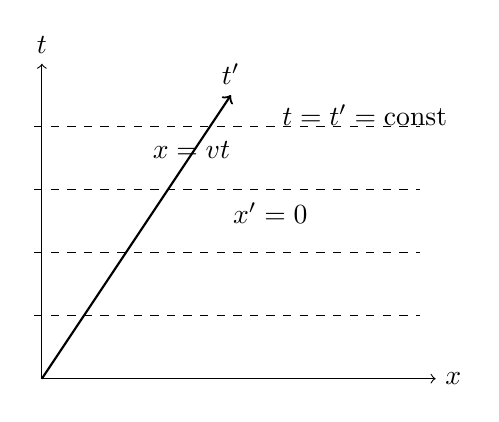
\begin{tikzpicture}[x=1cm,y=1cm]
\draw[->] (0,0) -- (0,4) node[above] {$t$};
\draw[->] (0,0) -- (5,0) node[right] {$x$};
\draw[thick,->] (0,0) -- (2.4,3.6) node[above] {$t'$};

\draw[dashed] (-0.1,0.8) -- (4.8,0.8);
\draw[dashed] (-0.1,1.6) -- (4.8,1.6);
\draw[dashed] (-0.1,2.4) -- (4.8,2.4);
\draw[dashed] (-0.1,3.2) -- (4.8,3.2);

\node at (1.9,2.9) {$x=vt$};
\node at (2.9,2.1) {$x'=0$};
\node at (4.1,3.35) {$t=t'=\mathrm{const}$};
\end{tikzpicture}
\caption{The opening board setup for the Galilean review, followed by a clean reconstruction of the spacetime picture described in the lecture. The moving origin traces the slanted line \(x=vt\), while constant-\(t\) and constant-\(t'\) slices coincide.}
\end{figure}

This is the baseline that Einstein will disturb. One should see exactly where the old intuition lives before one says what replaces it.

\section{From Galileo to Lorentz}

The point of failure is simple. Galilean relativity is incompatible with the statement that the speed of light is the same in every inertial frame. The correction is the Lorentz transformation:
\begin{align}
x' &= \frac{x-vt}{\sqrt{1-v^2}}, &
t' &= \frac{t-vx}{\sqrt{1-v^2}},
\end{align}
where for the moment we have set \(c=1\). Restoring dimensions gives
\begin{align}
x' &= \frac{x-vt}{\sqrt{1-v^2/c^2}}, &
t' &= \frac{t-vx/c^2}{\sqrt{1-v^2/c^2}}.
\end{align}
Two features should be emphasized immediately.

First, when \(v \ll c\), the correction is tiny:
\begin{equation}
\sqrt{1-\frac{v^2}{c^2}} \approx 1.
\end{equation}
In that limit we recover the Galilean formulas to excellent accuracy. Relativity does not abolish Newton; it contains Newton as the slow-velocity approximation.

Second, something genuinely new has happened to time. The formula for \(x'\) looks like Galileo with a denominator attached. The formula for \(t'\) is deeper: time is no longer shared universally. Space and time now mix.

For motion along the \(x\)-axis, the transverse coordinates are spectators:
\begin{equation}
y'=y, \qquad z'=z.
\end{equation}
Only the coordinate along the direction of motion mixes with time.

\subsection{Question \& Answer}

\paragraph{Question.} Why do \(y\) and \(z\) remain unchanged when \(x\) and \(t\) get mixed together? And what exactly is the invariant content of the meter-stick argument?

\paragraph{Answer.} Susskind's argument is deliberately operational. Imagine two meter sticks oriented transversely to the motion, one moving and one at rest, passing each other. In a frame halfway between them the situation is symmetric: each stick approaches with the same speed, so there is no distinguished reason for one to appear shorter than the other in the transverse direction. The symmetry therefore forbids any transverse contraction.

But the more basic statement is about events. If the ends of two objects coincide at one spacetime point in one frame, then that coincidence is an event, and the event is frame-independent. A flash of light may mark it, but the flash is only evidence; the invariant object is the spacetime coincidence itself. Thus the meeting of endpoints is not something one frame can regard as real while another frame denies it. This is why the meter-stick thought experiment can be trusted: it is ultimately an argument about shared events, not about visual impression alone.

\section{Light-Cone Coordinates and the Geometry of Lorentz Transformations}

At this stage Susskind changes register. Instead of introducing a new formula, he rewrites the same formula in a way that makes the geometry visible. Set \(c=1\) and add the two Lorentz equations:
\begin{align}
t'+x'
&= \frac{(t-vx)+(x-vt)}{\sqrt{1-v^2}} \\
&= \frac{(t+x)(1-v)}{\sqrt{1-v^2}} \\
&= (t+x)\sqrt{\frac{1-v}{1+v}}.
\end{align}
Now subtract:
\begin{align}
t'-x'
&= \frac{(t-vx)-(x-vt)}{\sqrt{1-v^2}} \\
&= \frac{(t-x)(1+v)}{\sqrt{1-v^2}} \\
&= (t-x)\sqrt{\frac{1+v}{1-v}}.
\end{align}

This is the cleanest algebraic form of the Lorentz transformation. The combinations
\begin{equation}
t+x, \qquad t-x
\end{equation}
are coordinates along the two \(45^\circ\) null directions, the directions followed by light rays in a spacetime diagram with \(c=1\). Under a Lorentz transformation, each null coordinate is merely multiplied by a factor, and the two factors are inverses of one another.

That is the geometric punchline: a Lorentz transformation is a squeeze. One lightlike direction is compressed, the other is stretched by the reciprocal amount. What does not change are the light rays themselves. The \(45^\circ\) directions remain \(45^\circ\). This is exactly what it means for light to have the same speed in every inertial frame.

The lecture's order matters here. One does not yet talk about proper time. One first learns to see Lorentz transformations as geometric operations on the light cone.

\section{Proper Time as the Invariant Interval}

Now comes the next shift. In Euclidean geometry, if one rotates coordinates from \((x,y)\) to \((x',y')\), the invariant quantity is the squared distance
\begin{equation}
s^2 = x^2+y^2 = x'^2+y'^2.
\end{equation}
Special relativity has an analogous invariant, but with a minus sign:
\begin{equation}
t'^2-x'^2 = t^2-x^2.
\end{equation}

\begin{proposition}
Under the Lorentz transformation in \(1+1\) dimensions, the quantity \(t^2-x^2\) is invariant.
\end{proposition}

\begin{proof}
Starting from
\begin{equation}
x'=\frac{x-vt}{\sqrt{1-v^2}},
\qquad
t'=\frac{t-vx}{\sqrt{1-v^2}},
\end{equation}
we compute
\begin{align}
t'^2-x'^2
&= \frac{(t-vx)^2-(x-vt)^2}{1-v^2} \\
&= \frac{t^2-2tvx+v^2x^2-x^2+2xvt-v^2t^2}{1-v^2} \\
&= \frac{(1-v^2)t^2-(1-v^2)x^2}{1-v^2} \\
&= t^2-x^2.
\end{align}
The cross terms cancel, and the remaining common factor \(1-v^2\) drops out.
\end{proof}

In three spatial dimensions the same invariant becomes
\begin{equation}
t'^2-x'^2-y'^2-z'^2 = t^2-x^2-y^2-z^2.
\end{equation}
For the lecture, the \(x\)-direction is the active one and \(y,z\) are usually suppressed, but the full statement is worth keeping in view.

\begin{definition}
If one event is the origin and a second event lies in the time-like region, its proper time from the origin is
\begin{equation}
\tau=\sqrt{t^2-x^2}
\end{equation}
in \(c=1\) units. More generally, for two nearby events one uses the same expression with coordinate differences:
\begin{equation}
\Delta \tau^2 = \Delta t^2-\Delta x^2-\Delta y^2-\Delta z^2.
\end{equation}
\end{definition}

Why the square root? Because the analogy is with ordinary distance. In Euclidean geometry, distance is the square root of the invariant quadratic form. Here the invariant quadratic form has the opposite sign in the spatial directions, but the logic is the same.

The sign difference changes the geometry dramatically. If \(t^2>x^2\), then \(\tau\) is real. If \(t^2=x^2\), then \(\tau=0\). If \(t^2<x^2\), then the expression under the square root is negative. In the lecture Susskind says, quite bluntly, that the proper time is then imaginary. For polished notes it is better to say that the interval is space-like, but the warning is the same: not every separation behaves like elapsed clock time.

\begin{figure}[h]
\centering
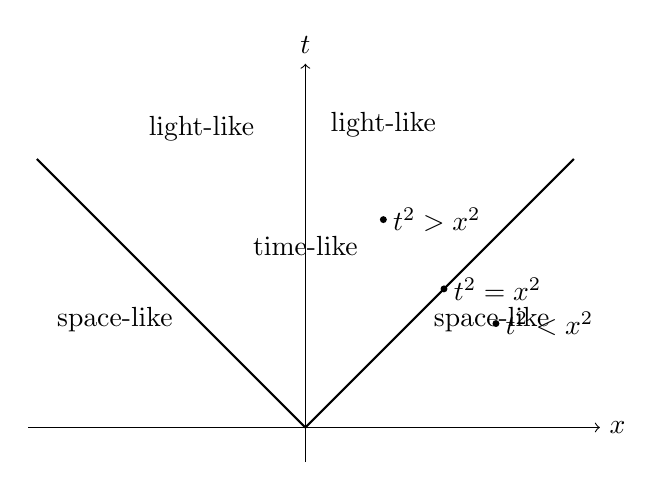
\begin{tikzpicture}[x=1.1cm,y=1.1cm]
\draw[->] (-3.2,0) -- (3.4,0) node[right] {$x$};
\draw[->] (0,-0.4) -- (0,4.2) node[above] {$t$};

\draw[thick] (0,0) -- (3.1,3.1);
\draw[thick] (0,0) -- (-3.1,3.1);

\node at (0.9,3.5) {light-like};
\node at (-1.2,3.45) {light-like};
\node at (0,2.1) {time-like};
\node at (2.15,1.25) {space-like};
\node at (-2.2,1.25) {space-like};

\draw[dashed] (0,0) -- (0,3.2);
\fill (0.9,2.4) circle (0.04);
\fill (2.2,1.2) circle (0.04);
\fill (1.6,1.6) circle (0.04);

\node[right] at (0.9,2.4) {$t^2>x^2$};
\node[right] at (1.6,1.6) {$t^2=x^2$};
\node[right] at (2.2,1.2) {$t^2<x^2$};
\end{tikzpicture}
\caption{The light cone in \(1+1\) dimensions. Inside the cone the interval is time-like and the proper time is real; on the cone the proper time is zero; outside the cone the separation is space-like.}
\end{figure}

The operational meaning now follows quickly. For a clock at rest in the unprimed frame, \(x=0\), so
\begin{equation}
\tau=\sqrt{t^2}=t.
\end{equation}
Thus proper time agrees with ordinary clock time for an observer at rest.

For a moving object, the principle of relativity says we may go to the frame in which that object is at rest. Along its worldline \(x'=0\), and then
\begin{equation}
\tau=\sqrt{t'^2-x'^2}=t'.
\end{equation}
So a moving wristwatch reads proper time. That is the physical meaning of the invariant interval.

\section{Time Dilation and Relativity of Simultaneity}

To derive time dilation, Susskind returns to the simplest possible worldline: the moving observer's own origin. In the unprimed coordinates that worldline is
\begin{equation}
x=vt.
\end{equation}
In the primed coordinates it is simply \(x'=0\).

\begin{figure}[h]
\centering

\includegraphics[width=0.54\textwidth]{lecture_04_figure_03.png}

\vspace{1em}

\begin{tikzpicture}[x=1cm,y=1cm]
\draw[->] (0,0) -- (0,4) node[above] {$t$};
\draw[->] (0,0) -- (5,0) node[right] {$x$};

\draw[thick,->] (0,0) -- (2.35,3.6) node[above] {$t'$};
\node at (1.45,2.85) {$x=vt$};
\node at (3.1,2.0) {$x'=0$};

\fill (1.75,2.68) circle (0.04);
\draw[dashed] (1.75,2.68) -- (0,2.68);
\node[left] at (0,2.68) {$t$};
\end{tikzpicture}
\caption{The photographed board and a clean reconstruction of the same point: the moving clock lies on the slanted worldline \(x=vt\), which is precisely the locus \(x'=0\). In the primed frame this line is the time axis.}
\end{figure}

Now use the invariance of proper time:
\begin{equation}
t'^2-x'^2=t^2-x^2.
\end{equation}
Along the moving clock's worldline, \(x'=0\) and \(x=vt\). Therefore
\begin{align}
t'^2 &= t^2-x^2 \\
&= t^2-v^2t^2 \\
&= (1-v^2)t^2.
\end{align}
Taking the positive square root,
\begin{equation}
t' = t\sqrt{1-v^2}.
\end{equation}
This is the time-dilation formula in units with \(c=1\). Restoring dimensions,
\begin{equation}
t' = t\sqrt{1-\frac{v^2}{c^2}}.
\end{equation}

The interpretation is direct. Between the same two events, the moving clock records less elapsed time than the stationary grid of synchronized clocks. A moving clock runs slow.

\subsection{Question \& Answer}

\paragraph{Question.} How can there be complete symmetry between the two inertial observers if each one says that the other clock runs slow?

\paragraph{Answer.} Because the two observers are not comparing the same pairs of events. The stationary observer uses horizontal slices \(t=\mathrm{const}\). The moving observer uses tilted slices \(t'=\mathrm{const}\). From
\begin{equation}
t'=\frac{t-vx}{\sqrt{1-v^2}},
\end{equation}
we see that holding \(t'\) fixed means
\begin{equation}
t-vx=\mathrm{const}.
\end{equation}
So the moving observer's simultaneity slices are not horizontal at all.

\begin{figure}[h]
\centering
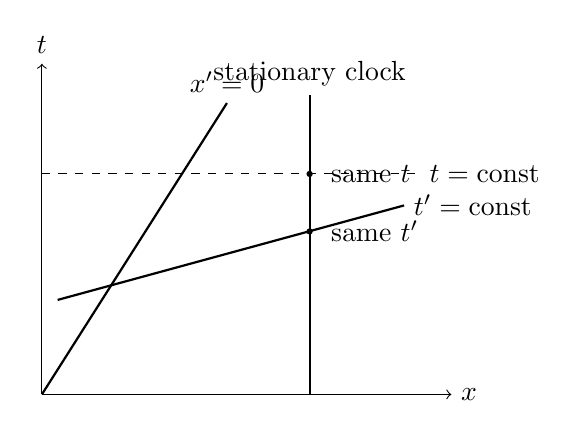
\begin{tikzpicture}[x=1cm,y=1cm]
\draw[->] (0,0) -- (0,4.2) node[above] {$t$};
\draw[->] (0,0) -- (5.2,0) node[right] {$x$};

\draw[thick] (0,0) -- (2.35,3.7) node[above] {$x'=0$};

\draw[dashed] (0,2.8) -- (4.8,2.8);
\node[right] at (4.8,2.8) {$t=\mathrm{const}$};

\draw[thick] (0.2,1.2) -- (4.6,2.4);
\node[right] at (4.6,2.4) {$t'=\mathrm{const}$};

\draw[thick] (3.4,0) -- (3.4,3.8);
\node[above] at (3.4,3.8) {stationary clock};

\fill (3.4,2.8) circle (0.04);
\fill (3.4,2.07) circle (0.04);

\node[right] at (3.55,2.8) {same \(t\)};
\node[right] at (3.55,2.07) {same \(t'\)};
\end{tikzpicture}
\caption{Relativity of simultaneity. A stationary observer compares readings on a horizontal slice \(t=\mathrm{const}\), while the moving observer compares readings on a tilted slice \(t'=\mathrm{const}\). The two claims about ``the other clock'' therefore refer to different pairs of events.}
\end{figure}

This is not a loophole; it is the content of relativity of simultaneity. The reciprocity of time dilation survives because the reciprocity of Lorentz transformations survives.

\section{Twin Paradox, Ideal Clocks, and Signal Exchange}

Once proper time is understood as the time read by a clock carried along a worldline, the twin paradox becomes almost routine. Let one twin remain at rest and let the other travel outward at speed \(v\), turn around, and return at the same speed. If the stay-at-home twin measures a time \(T\) on the outgoing leg and another time \(T\) on the return leg, then the home twin's elapsed time is
\begin{equation}
\tau_{\mathrm{home}} = 2T.
\end{equation}
For the traveling twin, one leg has
\begin{equation}
x=vT,
\qquad
\tau_{\mathrm{leg}}^2 = T^2 - v^2T^2 = (1-v^2)T^2,
\end{equation}
so
\begin{equation}
\tau_{\mathrm{leg}} = T\sqrt{1-v^2}.
\end{equation}
The round trip therefore gives
\begin{equation}
\tau_{\mathrm{travel}} = 2T\sqrt{1-v^2}.
\end{equation}
Because \(1-v^2<1\), the traveling twin ages less.

\begin{figure}[h]
\centering
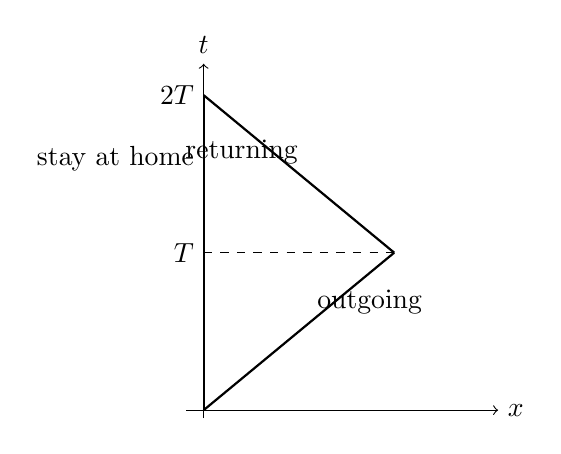
\begin{tikzpicture}[x=1.1cm,y=1cm]
\draw[->] (-0.2,0) -- (3.4,0) node[right] {$x$};
\draw[->] (0,-0.1) -- (0,4.4) node[above] {$t$};

\draw[thick] (0,0) -- (0,4);
\draw[thick] (0,0) -- (2.2,2);
\draw[thick] (2.2,2) -- (0,4);

\draw[dashed] (0,2) -- (2.2,2);

\node[left] at (0,2) {$T$};
\node[left] at (0,4) {$2T$};
\node[above right] at (1.2,1.1) {outgoing};
\node[above left] at (1.2,3.0) {returning};
\node[left] at (0,3.2) {stay at home};
\end{tikzpicture}
\caption{Twin paradox as a comparison of proper times along two worldlines: one straight and one broken. The clocks do not disagree about geometry; they record different lengths in spacetime.}
\end{figure}

The lecture is careful not to leave the calculation at the level of slogan. The point is not merely that a formula says so. The point is that clocks measure proper time, and proper time along the broken path is smaller than along the straight vertical path.

\subsection{Question \& Answer}

\paragraph{Question.} Does acceleration invalidate the twin-paradox calculation? After all, the turnaround is not an inertial segment.

\paragraph{Answer.} The acceleration is real, and one should not pretend otherwise. But two separate issues must be distinguished.

First, the sharp corner in the spacetime diagram is only an idealization. One may smooth it into a finite turnaround without changing the conclusion.

Second, the physical assumption is that a sufficiently good clock is an ideal clock: modest acceleration does not materially alter its rate, so it continues to tick off proper time. Then a curved worldline can be divided into many short pieces, each nearly inertial, and the total elapsed time is obtained by adding the segment-by-segment proper times:
\begin{equation}
\tau_{\mathrm{path}} \approx \sum_i \sqrt{\Delta t_i^2-\Delta x_i^2}.
\end{equation}
This is the spacetime analogue of computing the length of an ordinary curve by chopping it into short straight segments.

The lecture is explicit that this ideal-clock assumption is a physical assumption, not a theorem proved from the preceding algebra alone. Big, sloppy clocks can break under acceleration. Small, well-built clocks can be made faithful enough that the relativistic geometry is what they report.

The discussion then shifts from formal proper times to what observers actually receive. Imagine each twin emitting one light pulse every second of his or her own proper time. On the outward leg the pulses are received more sparsely; on the return leg they arrive bunched together. This is the Doppler-style operational picture that accompanies the geometry. Nothing goes missing. Each observer eventually receives every pulse sent by the other, but the arrival rates depend on the changing relative motion.

A related question about energy is raised and then postponed. Susskind is careful here: the lecture at this stage is about \(x\)'s and \(t\)'s, not yet about the full relativistic energetics of accelerated observers.

\subsection{Question \& Answer}

\paragraph{Question.} Suppose one spatial direction were compact, so that an observer could move uniformly around a closed loop and return without the usual turn-around. Would there still be an asymmetry?

\paragraph{Answer.} The lecture keeps this question open rather than polishing it into a theorem. The claim is that there is still an asymmetry, because the observer moving around the compact direction can discover operationally that the direction is special: one repeatedly returns to the same places. But Susskind explicitly declines to give a finished derivation on the spot. The right way to preserve this moment is to record the qualitative point and to leave the geometry provisional.

\begin{figure}[h]
\centering

\includegraphics[width=0.56\textwidth]{lecture_04_figure_04.png}
\caption{The later board at the compact-direction discussion. The algebra on the left is too fragmentary to transcribe cleanly, but the right-hand geometric sketch records that the lecture had shifted to an asymmetry puzzle rather than a finished derivation.}
\end{figure}

\begin{figure}[h]
\centering
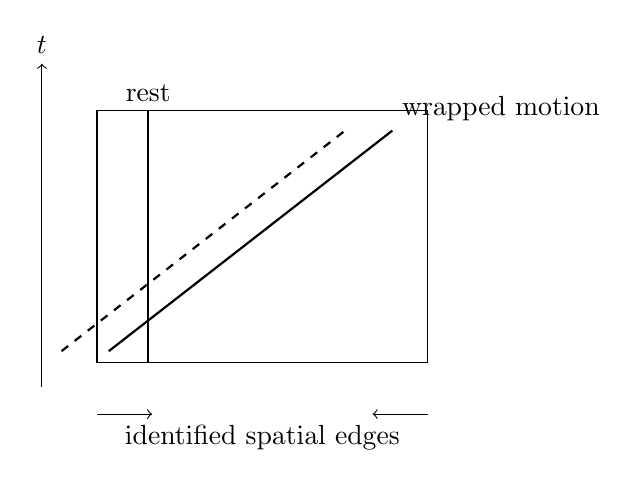
\begin{tikzpicture}[x=1cm,y=1cm]
\draw[->] (0,0) -- (0,4.1) node[above] {$t$};
\draw (0.7,0.3) rectangle (4.9,3.5);

\draw[->] (0.7,-0.35) -- (1.4,-0.35);
\draw[->] (4.9,-0.35) -- (4.2,-0.35);
\node at (2.8,-0.65) {identified spatial edges};

\draw[thick] (1.35,0.3) -- (1.35,3.5);
\node[above] at (1.35,3.5) {rest};

\draw[thick] (0.85,0.45) -- (4.45,3.25);
\draw[thick,dashed] (0.25,0.45) -- (3.85,3.25);
\node[above right] at (4.45,3.25) {wrapped motion};
\end{tikzpicture}
\caption{A cautious schematic reconstruction of the compact-direction question, drawn on an unwound strip. This is not a settled result of the lecture; it only records the qualitative asymmetry that was being discussed.}
\end{figure}

\section{Length Contraction}

The lecture now returns to a problem Susskind wants to do in the same spirit as time dilation. His advice is emphatic: always draw a picture.

Take a meter stick at rest in the unprimed frame. Its left end sits at \(x=0\), its right end at \(x=1\). As time passes, these two endpoints sweep out a ribbon in spacetime: two vertical worldlines separated by one unit of \(x\).

Now ask what the moving observer means by the rod's length. The answer is not the unprimed separation of arbitrary points on the ribbon. The moving observer must compare the two endpoints at the same instant of the moving observer's own time. That means one must intersect the rod's spacetime ribbon with a constant-\(t'\) slice.

For the special slice \(t'=0\), the Lorentz transformation tells us
\begin{equation}
t-vx=0,
\end{equation}
so along that slice,
\begin{equation}
t=vx.
\end{equation}
In particular, where the slice meets the right endpoint worldline \(x=1\), the corresponding unprimed time is
\begin{equation}
t=v.
\end{equation}

\begin{figure}[h]
\centering
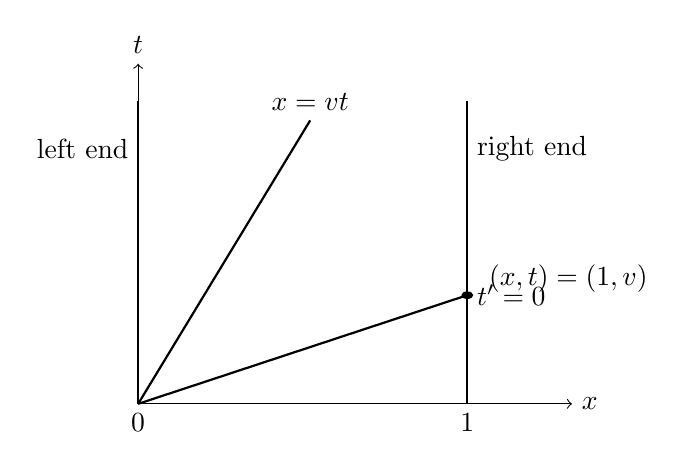
\begin{tikzpicture}[x=1.9cm,y=1.2cm]
\draw[->] (0,0) -- (0,3.6) node[above] {$t$};
\draw[->] (0,0) -- (2.9,0) node[right] {$x$};

\draw[thick] (0,0) -- (0,3.2);
\draw[thick] (2.2,0) -- (2.2,3.2);
\node[below] at (0,0) {$0$};
\node[below] at (2.2,0) {$1$};

\draw[thick] (0,0) -- (1.15,3.0);
\node[above] at (1.15,3.0) {$x=vt$};

\draw[thick] (0,0) -- (2.2,1.15);
\node[right] at (2.2,1.15) {$t'=0$};

\fill (2.2,1.15) circle (0.04);
\node[right] at (2.28,1.33) {$(x,t)=(1,v)$};

\node[right] at (2.2,2.7) {right end};
\node[left] at (0,2.7) {left end};
\end{tikzpicture}
\caption{Length contraction from a spacetime picture. The rod is at rest in the unprimed frame, so its endpoints trace vertical worldlines. The moving observer measures the rod by intersecting that ribbon with a single constant-\(t'\) slice.}
\end{figure}

Now use the same invariant interval as before. For the point where the \(t'=0\) slice hits the right endpoint, the primed interval from the origin is
\begin{equation}
t'^2-x'^2 = -x'^2,
\end{equation}
because \(t'=0\). In the unprimed frame, the same point has coordinates \(x=1\) and \(t=v\), so
\begin{equation}
t^2-x^2 = v^2-1 = -(1-v^2).
\end{equation}
Equating the two expressions gives
\begin{equation}
-x'^2 = -(1-v^2),
\end{equation}
hence
\begin{equation}
x'=\sqrt{1-v^2}.
\end{equation}
Therefore a rod of rest length \(1\) is seen in the moving frame to have length
\begin{equation}
L'=\sqrt{1-v^2}.
\end{equation}
For a general rest length \(L\),
\begin{equation}
L' = L\sqrt{1-v^2}
\end{equation}
in units with \(c=1\), or
\begin{equation}
L' = L\sqrt{1-\frac{v^2}{c^2}}
\end{equation}
when \(c\) is restored.

This is the same geometry seen from the other side. Time dilation came from following one moving worldline. Length contraction comes from slicing a stationary ribbon with the moving observer's simultaneity plane. Both are statements about how Lorentz transformations mix space and time.

The lecture closes by immediately turning this into an operational point about travel. If distant stars are Lorentz-contracted in the astronaut's frame, then the astronaut may cross the gap in a shorter proper time without anything moving faster than light. The stars do not rush by superluminally; they remain subluminal objects seen in a frame where the spatial separation has changed.

\section{Summary}

The lecture begins with Galileo on purpose. In the Galilean picture the moving origin tilts but time slices remain horizontal. Einstein's correction changes that: \(x\) and \(t\) mix, the light cone is preserved, and the invariant quantity is no longer \(x^2+y^2\) but \(t^2-x^2-y^2-z^2\).

From that one invariant, the rest follows in the order Susskind insists on. Proper time is the time read by a clock carried along a worldline. Moving clocks run slow because the proper time between two events is smaller than the coordinate time in a frame relative to which the clock moves. The twin paradox is not a paradox once one compares proper times along different paths. Length contraction is the companion effect obtained by taking a moving observer's simultaneity slice through the spacetime ribbon of a rod.

What the lecture ultimately teaches is not a list of isolated formulas but a habit of thought: draw the spacetime picture, identify the invariant quantity, and let the geometry tell you what clocks and rods will do.